
\subsubsection{Pure Pursuit}
\label{sect:pure-pursuit}
In this section we describe a popular and simple method from the class of geometric path tracking algorithms. 

We provide a brief informal sketch of the algorithm, and then detail its relation to the inputs of the velocity and steering tracking controllers.

\textbf{Algorithm:}
\begin{itemize}
	\item Update vehicle state
	\item Find nearest path point
	\item Find the goal point
	\item Transform goal to vehicle coordinates
	\item Calculate desired curvature
	\item Set steering to desired curvature
	\item Update position
\end{itemize}

While the pure pursuit algorithm is simple and effective, in practice it has the downside that the requested steering angles are not continuous. This results in unnatural steering which occupants may perceive to be jerky. We utilize this method because it provides a simple closed form solution which can be easily modeled in current hybrid systems verification tools. In Section \ref{sect:extensions} we discuss alternatives which may be tractable within the framework developed in these benchmarks.

\begin{figure}
	\centering
	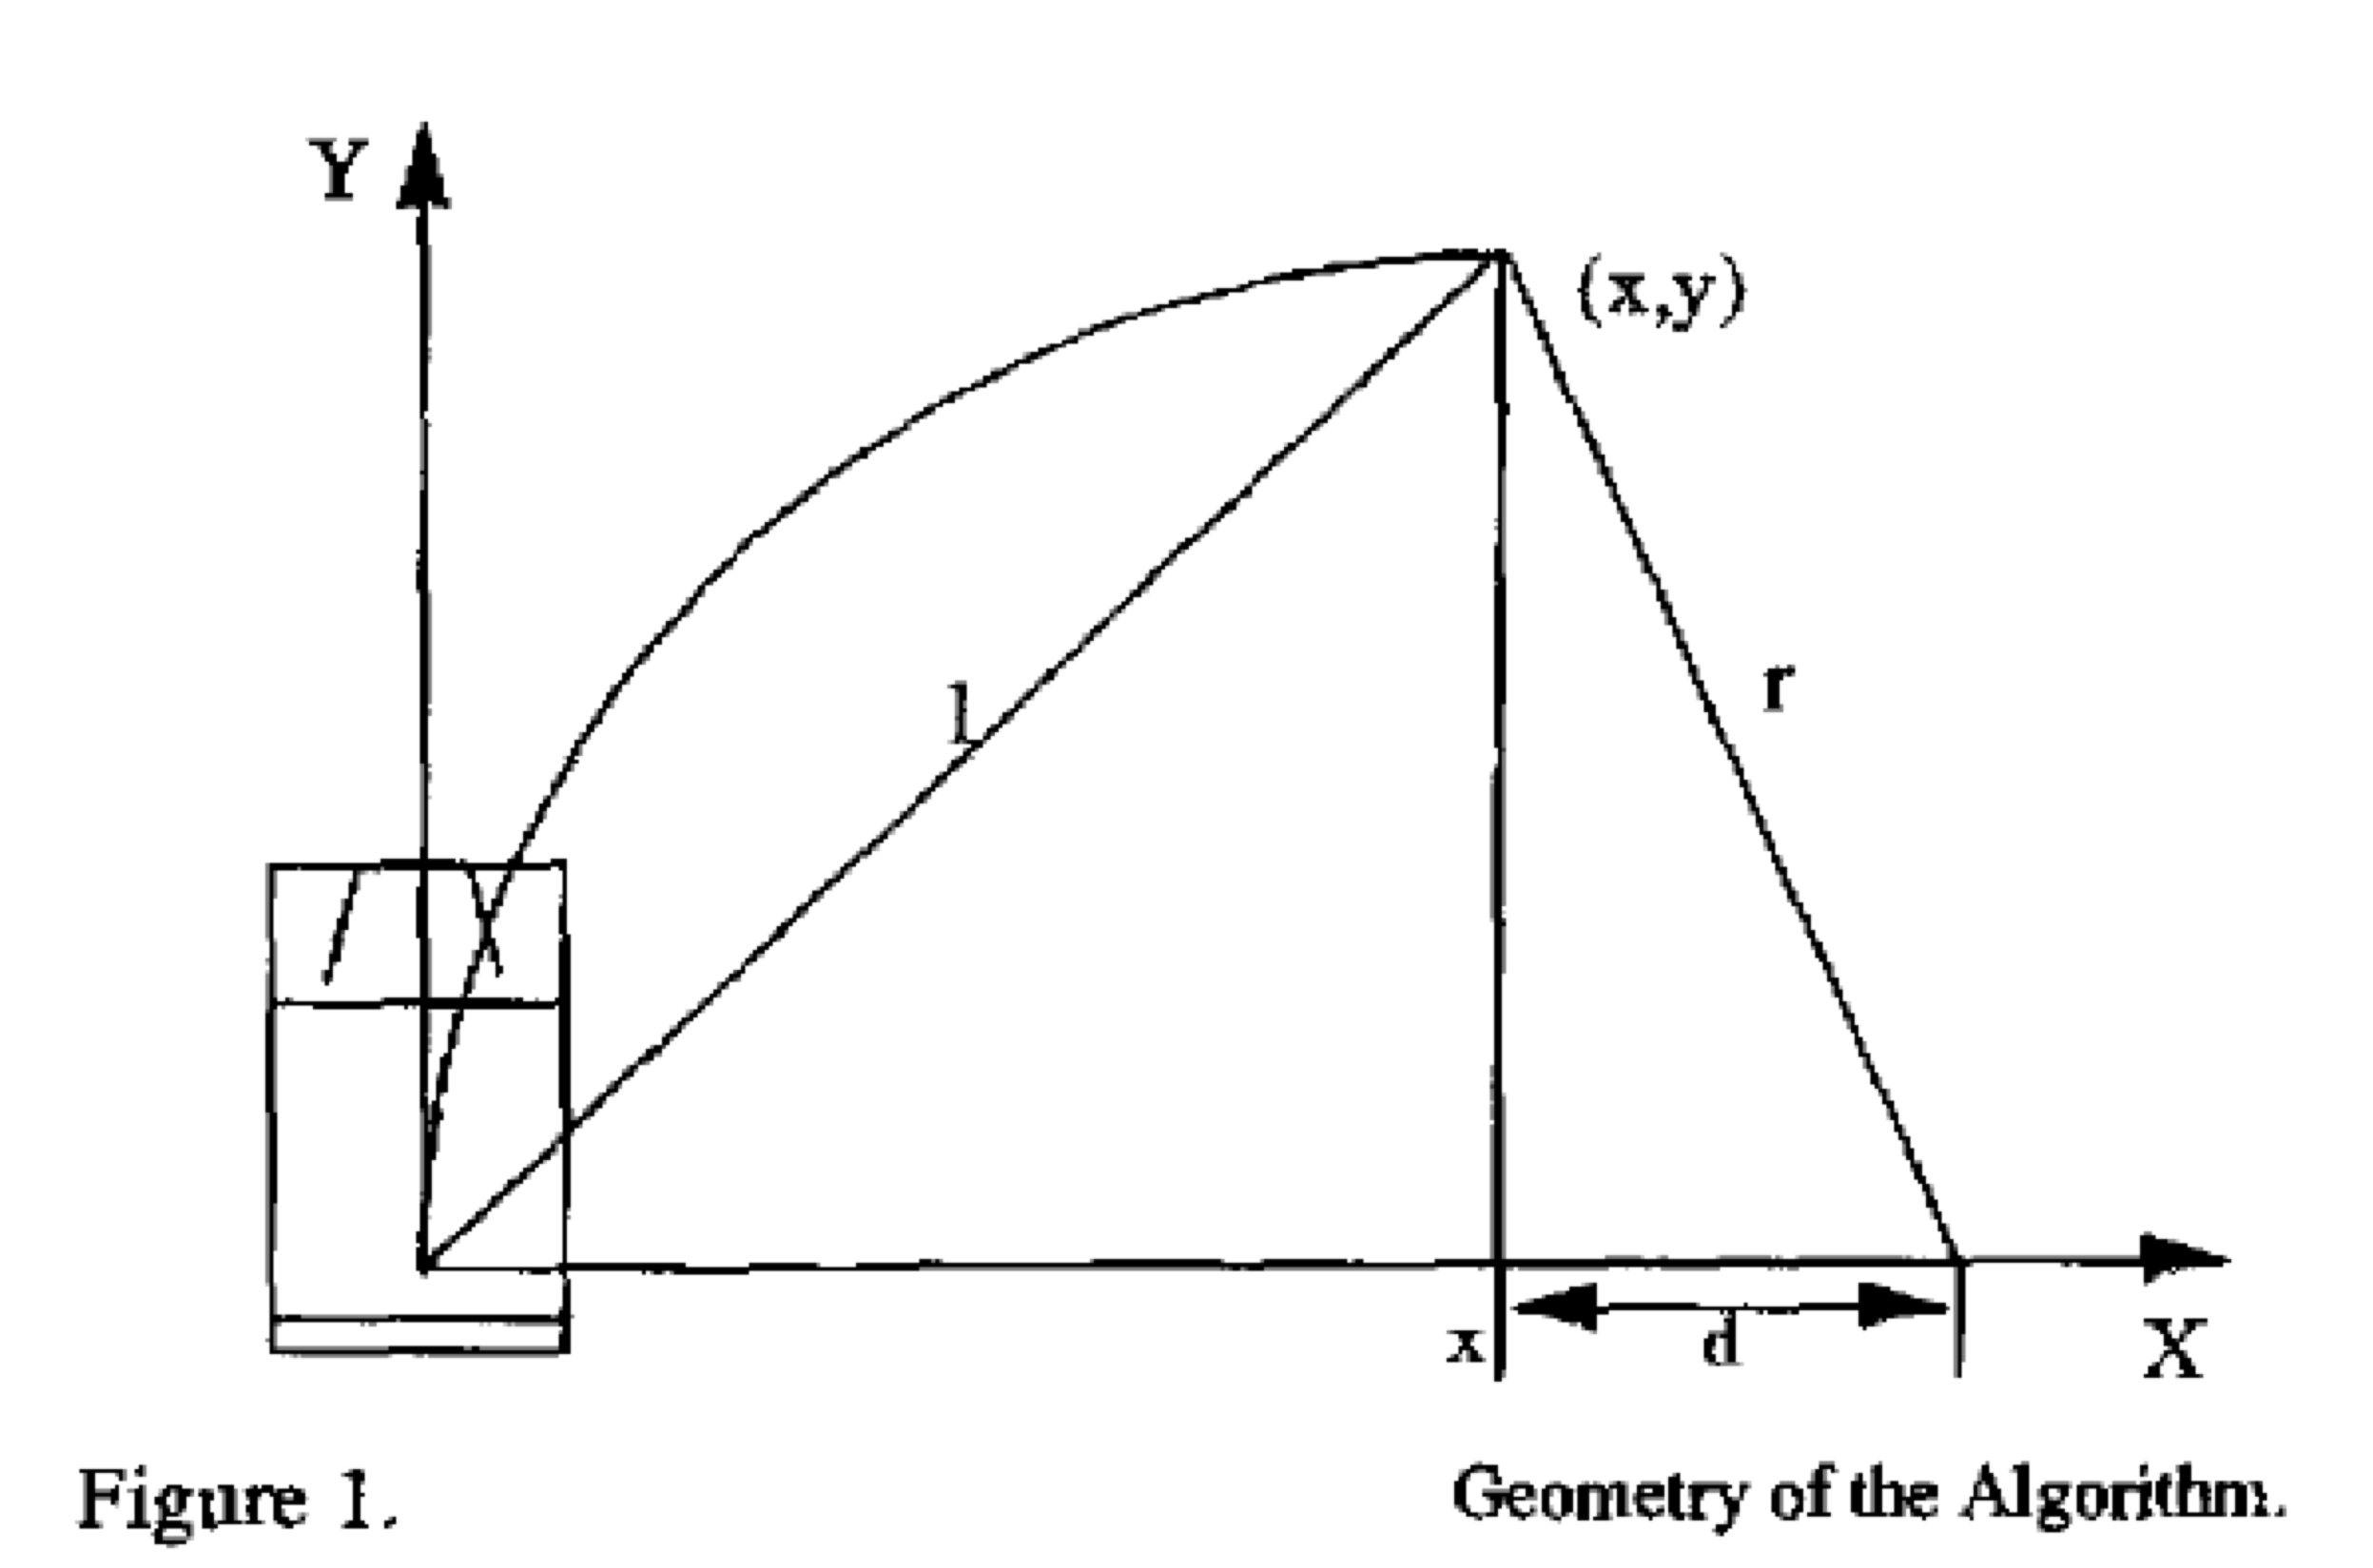
\includegraphics[scale=.5]{figures/pure_pursuit_geom}
	\caption{Geometry of Pure Pursuit Algorithm}
\end{figure}

\noindent Given the relations: $x^2+y^2=l^2$ and $x+d=r$, the desired curvature is:
\begin{align}
\gamma=\frac{2x}{l^2}
\end{align}



%Thus, the feedback to the system are the lateral and longitudinal tracking errors. We derive the following results as in  \cite{Snider2009}:
%\begin{gather}
%	\epsilon_x=cos{(\Psi_d)}(s_{x,d}-s_x) +sin{(\Psi_d)}(s_{y,d}-s_y)
%	\\
%	\epsilon_y=-sin{(\Psi_d)}(s_{x,q}-s_x)+cos{(\Psi_d)}(s_{y,d}-s_y)
%\end{gather}

\noindent Thus, given the vehicle pose and the next waypoint. We must compute $\left\{\Psi_d, \dot{\Psi}_d, s_{x_d}, s_{y_d},\right\}$. 

This implies that:
\begin{equation}
	\theta(0) = sin^{-1} \left(\frac{s_y-c_y}{r}\right)
\end{equation}
Then we compute 
\begin{equation}
\Psi_d(t) =  \frac{\pi}{2}-\theta(t), t \geq 0
\end{equation}
For an arc subtended by the angle $\theta(t)$, the length of the arc, $\rho$ is:
\begin{equation}
	\rho = \theta(t) \cdotp r
\end{equation}
Alternately one might compute the length of the arc by integrating the velocity as directed along the arc such that $\rho(t) = \int_{0}^{t}v(\alpha) d\alpha$. Now we let $v(\alpha) = v_d$ and hold $v_d$ to be constant. Thus:
\begin{equation}
	\rho(t) = v_d \cdotp t
\end{equation}
Which implies that:
\begin{equation}
	\Psi_d(t) = \frac{\pi}{2} - \left( \theta(0) + \frac{v_d \cdotp t}{r}\right)
\end{equation}
Differentiating we conclude that:
\begin{equation}
	\dot{\Psi}_d = -\frac{v_d}{r}
\end{equation}
\begin{figure}
	\centering
	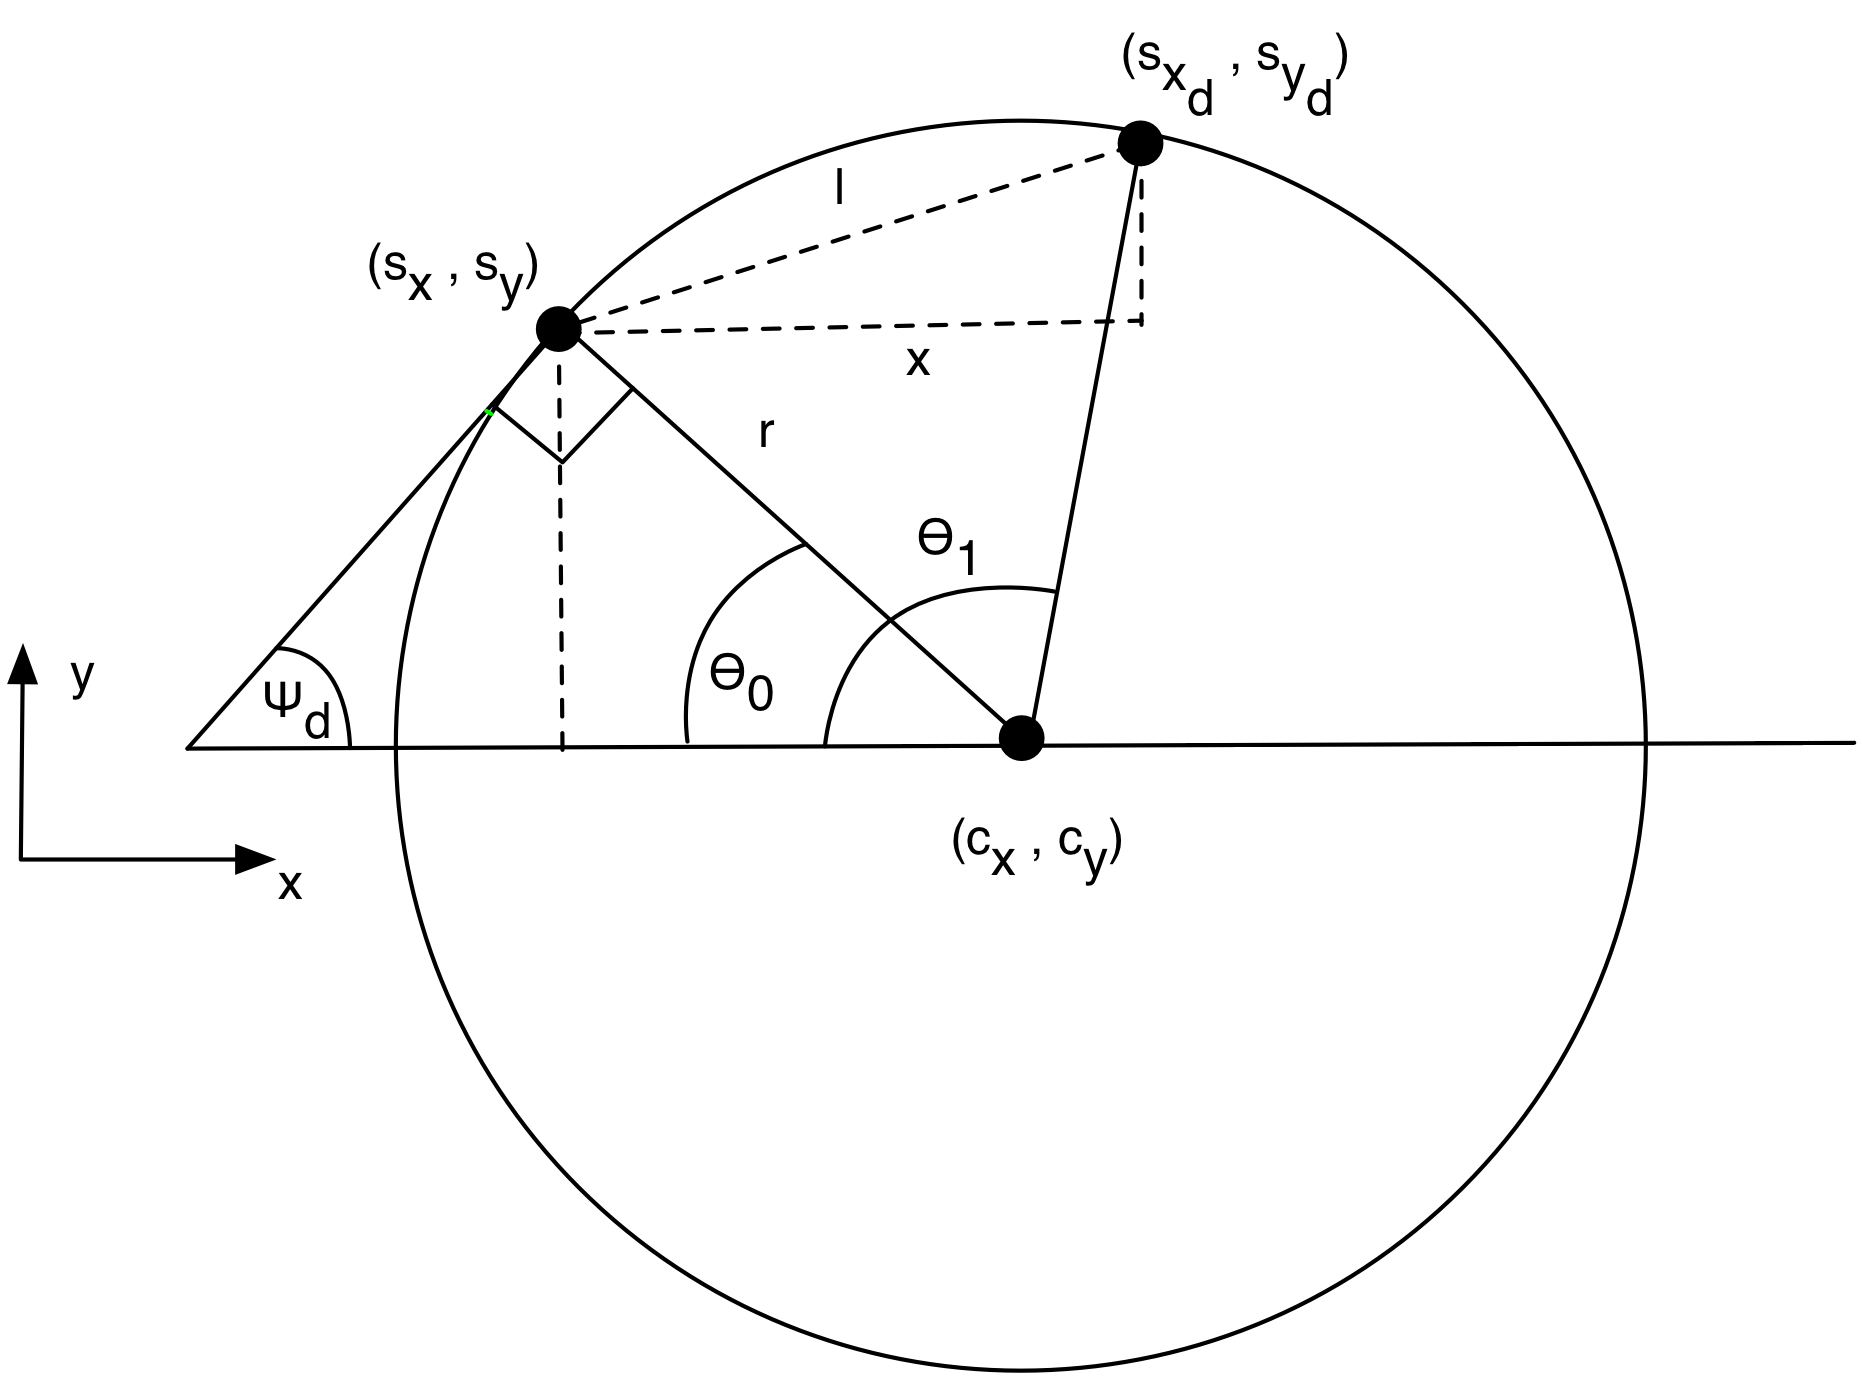
\includegraphics[scale=0.5]{figures/traj-track-diagram}
	\caption{Geometric Description of Ego-Vehicle Trajectory Geometry}
\end{figure}

\noindent Thus we can derive the remaining equations for a point mass moving in a plane:
\begin{gather}
 \dot{\Psi}_d= -v_d/r\\
 \dot{s}_{x_d} = v_d \left(cos(\Psi_d)\right)\\
 \dot{s}_{y_d} = v_d \left(sin(\Psi_d) \right)\\
 \ddot{\Psi}_d = 0
\end{gather}